\documentclass[12pt, a4paper]{article}
\usepackage[margin=0.5in]{geometry}

\usepackage{color}
\usepackage[dvipsnames]{xcolor}
\usepackage{hyperref}
\hypersetup{
    colorlinks=true,
    linkcolor=blue,
    urlcolor=blue,
    linktoc=all
}


\usepackage{amsmath}
\usepackage{mathtools}
\usepackage{amssymb}
\usepackage{cancel}
\usepackage{bm}
\usepackage{dsfont}
\usepackage{graphicx}
\usepackage{graphics}
\usepackage{xfrac}
\usepackage{array}
\setcounter{MaxMatrixCols}{40}

\usepackage{enumerate}
\usepackage{enumitem}
\usepackage{multirow}

%inclusions carried over from past class homework formats
\usepackage{units}
\usepackage{fullpage}
\usepackage{alltt}
\usepackage{mathrsfs}
\usepackage{xcolor}
\usepackage{soul}

\usepackage{pgfplots}

\DeclarePairedDelimiter{\abs}{\lvert}{\rvert}
\newcommand*{\fontCourier}{\fontfamily{pcr}\selectfont}
\newcommand*\mean[1]{\overline{#1}}
\newcommand\scalemath[2]{\scalebox{#1}{\mbox{\ensuremath{\displaystyle #2}}}}

\setcounter{tocdepth}{5}
\setcounter{secnumdepth}{5}

% \usepackage{pdfpages}
\usepackage{Sweave}
\begin{document}
% 
\includepdf{TitlePage_MastersThesis}
% 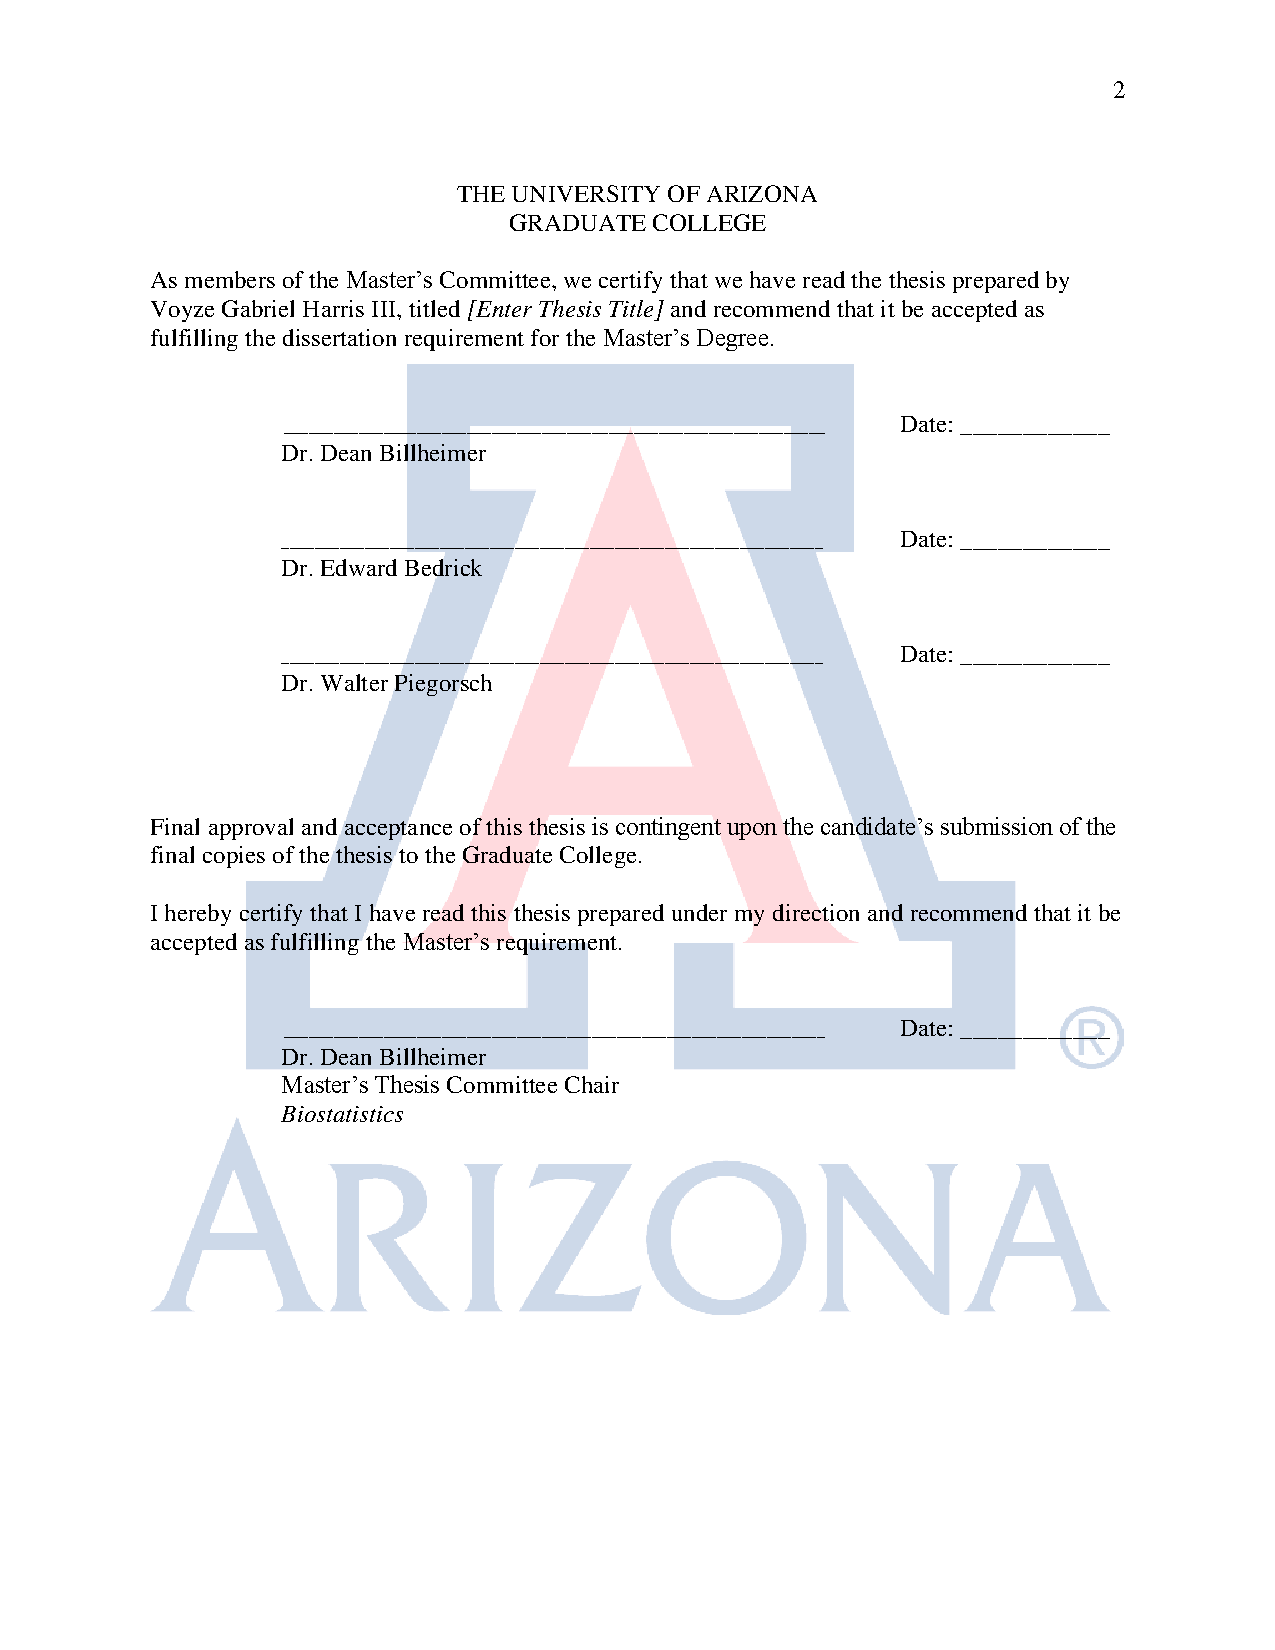
\includepdf{ThesisApprovalPage}
\Sconcordance{concordance:ToDoList.tex:ToDoList.Rnw:%
1 51 1 1 0 7 1 1 4 36 1}


% \tableofcontents
% \newpage



\title{To Do List}
\author{\Large Gabe Harris}
\maketitle

\begin{itemize}
  \item Read intros to listed texts (See Thesis section 2.1 Why Predictive Inference?) and summarize answers to that question in WhyPredictiveInference.Rnw
  \item Create example comparing predictive inference result with plug in parameter result
    \subitem Dean's suggestion:  1-sample binomial with small sample size.  E.g. 3 successes, 7 failures (Pr(success) < 0.5).  Difference will be more pronounced with smaller sample sizes.
  \item Combine rpredNormIG(), rpredNormIG2(), and rpredNormIGk() into one function
  \item Read up on convergence in probability and justification for MCMC (Hoff, Casella \& Berger)
  \item Compare variance computations: var() function on MCMC sample vs direct computation from theory ($EX^2 - (EX)^2$)
\end{itemize}











\end{document}
